\begin{frame}
    \frametitle{Test de Wilcoxon}
    Si bien, el test de signos puede cumplir la misma funcion que el de
    \textbf{Signos}, este ultimo tiene mayor potencia al momento de
    detectar diferencia de medias.
  
\end{frame}

\begin{frame}
    \frametitle{Prueba de Wilcoxon}
    Se realiza una prueba de Wilcoxon para 2 muestras
    \textbf{relacionadas} 
    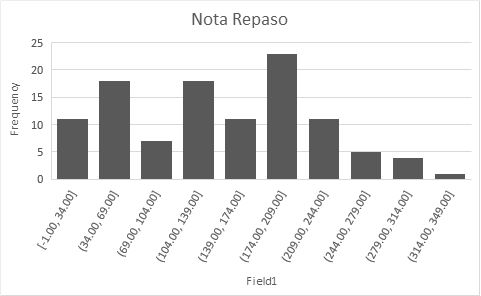
\includegraphics[width=1\textwidth]{cap/images/wilcoxon/repaso.jpg}
\end{frame}

\begin{frame}
    \frametitle{Prueba de Wilcoxon}
    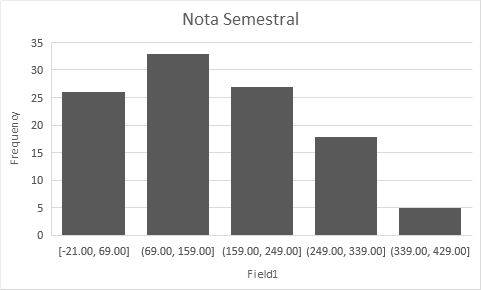
\includegraphics[width=1\textwidth]{cap/images/wilcoxon/semestral.jpg}
\end{frame}

\begin{frame}

    \frametitle{Prueba de Wilcoxon}

    \[H_0: \textrm{Las distribuciones son semejantes}\]
    
    \[H_1: \textrm{Las distribuciones se encuentran desplazadas}\]

    \[usando el test: Z_c = \frac{T_+ - \frac{[n(n + 1)]}{4}}{\sqrt{\frac{[n(n + 1)(2 * n + 1)]}{24}}}\]

\end{frame}

\begin{frame}

    Como se desea saber si el ciclo de repaso ayudó a mejorar los resultados 
    de aquellos estudiantes que estuvieron en el ciclo semestral.

    Dado que el estadistico de prueba: \[ Z = 2.991 \] es mayor al 
    \[Z_{crit} = 1.645\] se rechaza la hipotesis nula, por lo que se no
    se puede afirmar que ambas muestras sean identicas.

    \textbf{El repaso no ayudó a mejorar los conocimientos}
\end{frame}

\begin{frame}
    \frametitle{Prueba de Wilcoxon}
    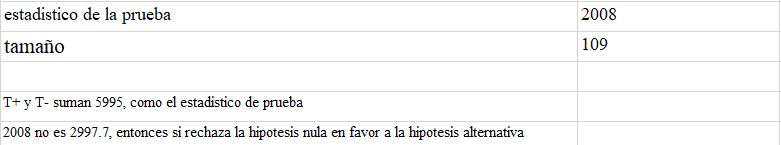
\includegraphics[width=1\textwidth]{cap/images/wilcoxon/resultados.jpg}
\end{frame}